\documentclass{article}
\usepackage[a4paper,margin=2.54cm]{geometry}
\usepackage[utf8]{inputenc}
\usepackage{natbib}
\usepackage{xcolor}
\usepackage{listings}
\usepackage{fancyhdr}
\usepackage{amsmath}
\usepackage[]{algorithm2e}
\usepackage{verbatim}
\usepackage{algorithm2e}
\usepackage{graphicx}
\usepackage{hyperref}
\usepackage[T1]{fontenc}

% Configuration pour les parties de code
% -----------------------------------
\lstdefinestyle{customc}{
  belowcaptionskip=1\baselineskip,
  breaklines=true,
  frame=L,
  xleftmargin=\parindent,
  language=C,
  showstringspaces=false,
  basicstyle=\footnotesize\ttfamily,
  keywordstyle=\bfseries\color{green!40!black},
  commentstyle=\itshape\color{purple!40!black},
  identifierstyle=\color{blue},
  stringstyle=\color{orange},
}

\lstdefinestyle{customasm}{
  belowcaptionskip=1\baselineskip,
  frame=L,
  xleftmargin=\parindent,
  language=[x86masm]Assembler,
  basicstyle=\footnotesize\ttfamily,
  commentstyle=\itshape\color{purple!40!black},
}
\lstset{escapechar=@,style=customc}

% Ecrire du code C en ligne de code

\newcommand{\inlinecode}[2]{\colorbox{white}{\lstinline[language=#1]$#2$}}

% -----------------------------------

% Indentation espacement
\setlength\parindent{24pt}

% Faire en sorte d'avoir plusieurs sous sections
\setcounter{secnumdepth}{4}

% Indiquer à Latex que l’on va utiliser les commandes internes
\makeatletter
\makeatother

% Renommer la table des matières
\renewcommand{\contentsname}{Table des matières}
\renewcommand{\listfigurename}{Table des figures}

% Faire en sorte que les liens hypertexte ne soient pas en rouge sur le document

\usepackage{hyperref}
\hypersetup{%
  colorlinks = true,
  linkcolor  = black
}

% Style des pages
\pagestyle{headings}

% Page de garde
\title{Projet de 1$^{ere}$ année : Shakespearian Monkeys}
\author{Laurent Genty - Florian Mornet}
\date{14 December 2018}

% Début du document
\begin{document}

% Page de garde
\begin{titlepage}

  \centering
  \scshape
  \vspace*{\baselineskip}
  \rule{\textwidth}{1.6pt}\vspace*{-\baselineskip}\vspace*{2pt}
  \rule{\textwidth}{0.4pt}
  \vspace{0.65\baselineskip}
  
  {\LARGE Projet de 1$^{ere}$ année : Programmation impérative}
    \vspace{0.60\baselineskip}
    
    {\LARGE Shakespearian Monkeys}
  \vspace{0.65\baselineskip}
  
  \rule{\textwidth}{0.4pt}\vspace*{-\baselineskip}\vspace{3.2pt}
  \rule{\textwidth}{1.6pt}
  \vspace{2\baselineskip}
  
  Générateur de texte aléatoire en C
  \vspace*{3\baselineskip}
  
  \begin{figure}[ht!]
    \centering
    
\includegraphics[scale=0.3]{logo.PNG}
    \label{fig:logo}
    \end{figure}
  
  \vspace{0.5\baselineskip}
  {\scshape\Large Laurent Genty \\ Florian Mornet \\}
  \vspace{0.5\baselineskip}
  \textit{ENSEIRB-Matmeca, Bordeaux}
  \vfill
  \vspace{0.3\baselineskip}
  
  14 Décembre 2018
\end{titlepage}



% ToC
\newpage
\tableofcontents

\listoffigures


% ------------------------ Introduction -------------------------
\newpage
\section{Introduction}
\label{sct:introduction}

% --- Objectifs principaux

\subsection{Objectifs principaux}
\label{subct:obj_principaux}

Ce projet a été réalisé dans le cadre du semestre 5 à l'ENSEIRB-Matmeca en programmation impérative. Il s'est déroulé du 23 octobre au 14 décembre par les élèves \textbf{Laurent Genty} et \textbf{Florian Mornet}, tous deux en formation d'ingénieur en informatique.

Les objectifs de ce projet sont nombreux. Tout d'abord, le but de ce projet est \textbf{de nous familiariser avec un langage} qui nous servira durant notre formation : \textbf{le C}. Mais pas seulement. En effet, un objectif majeur est de \textbf{construire une architecture solide et propice à une future évolution}, à savoir le rajout de fonctionnalités, d'idées avec le moins de difficultés possible.
Le projet s'étale sur plusieurs semaines avec plusieurs rendus possibles allant de la version de base aux différents \textit{achievements}. Le but étant d'aller le plus loin possible, mais en n'oubliant pas notre ligne directive qu'il vaille mieux \textbf{privilégier la qualité à la quantité} de code fourni.

% --- Sujet de base

\subsection{Sujet de base}
\label{sct:sujet_base}

Le sujet original est présent sur la site de M. Renault : \url{http://www.labri.fr/perso/renault/working/teaching/projets/s1-shakemonkeys.php}.

La version de base du projet consiste en la \textbf{reproduction d'un fichier sur la sortie standard}. Pour ce faire, nous devrons utiliser un système de singes ayant chacun des rôles différents afin de reproduire le texte. Il travailleront les uns à la suite des autres afin de faire avancer la reproduction du fichier. Voici la liste exhaustive de départ des singes à notre disposition :
\begin{itemize}
    \item \textbf{lecteur} : lire le fichier
    \item \textbf{imprimeur} : afficher les mots que le singe lecteur a lu
    \item \textbf{statisticien} : effectuer des statistiques sur les mots
\end{itemize}

Le jeu s'organisera en tours dans lesquels un singe travaillera et effectuera l'action appropriée. Une partie de jeu s'arrête lorsque tous les singes ont terminé leur travail pour de bon, ou bien qu'ils ont pris trop de temps et ont dépassé le nombre de tours limite. Nous expliquerons plus en détail un exemple type d'une partie de jeu mais pour faire simple : les singes sont choisis aléatoirement, travaillent et se mettent en grève pour qu'ensuite un autre singe travaille (et ainsi de suite).

Ce sujet, bien qu'anodin, nous permet de travailler sur différentes notions, comme par exemple :
\begin{itemize}
    \item pointeurs
    \item structures
    \item la gestion d'entrées sorties
    \item le développement de tests
\end{itemize}

% --- Remerciements

\subsection{Remerciements}
\label{sct:remerciements}

Avant de développer notre projet, nous tenons à remercier M. Mathieu Faverge, responsable de notre groupe durant la totalité de ce projet, et M. David Renault, responsable des projets de programmation lors de la première année de formation à l'ENSEIRB-Matmeca de nous avoir aidé et éclairé tout au long de ce projet.


% --------- Méthodologie et répartition des tâches --------------

\newpage
\section{Méthodologie et répartition des tâches}
\label{sct:methodo_taches}

Avant de foncer tête baissée dans le développement du programme, il était important de bien clarifier notre méthodologie de développement. À savoir :
\begin{enumerate}
    \item conception des structures
    \item se répartir les tâches
    \item commencer le développement
    \item effectuer les tests en parallèle
    \item écrire une documentation complète
\end{enumerate}

Bien évidemment ces tâches ne sont pas forcement linéaires. Il est possible que nous revenons à une certaine étape, puis ensuite repartir à une autre, etc...

% --- Modalités du rendu final

\subsection{Modalités du rendu final}
\label{subsct:modalite_rendu}

Concernant le rendu final, nous avions la possibilité de mettre les différentes versions du projet dans un dossier pour chaque et de créer donc des \textit{Makefile} associés.

Cependant, nous avons fait le choix de \textbf{travailler avec Git plus en profondeur}, notamment en \textbf{utilisant les branches}. D'un commun accord, nous avons décidé de développer toutes les versions sur une branche différente pour chaque dans la mesure où cela est beaucoup plus pratique en ce qui concerne le rendu, mais aussi pour la phase de développement : nous avons juste a changer de branche et le tour est joué. Mais les avantages sont doubles ! Cela nous fait travailler l'outil de gestionnaire de versions plus en profondeur, ce qui n'est pas négligeable.

\indent C'est donc pourquoi à l'heure où le projet a été rendu, nous avons :
\begin{itemize}
    \item \textbf{master} : version la plus avancée fonctionnelle
    \item \textbf{base} : code de la base version
    \item \textbf{achiev1} : code concernant l'achievement numéro 1
    \item \textbf{achiev2} : code pour l'achievement numéro 2
\end{itemize}

Malgré le fait qu'il soit rappelé dans le \textit{README}, il est important de le signaler afin que nous ne soyons pas pénalisés concernant la remise du projet le 14 décembre 2018.

% --- Répartition des tâches

\subsection{Répartition des tâches}
\label{subsct:taches}

Avant tout projet, il est important de savoir quelle personne souhaite effectuer quelle tâche en relation avec ce qu'il souhaite apprendre, ses forces et ses faiblesses. C'est donc pourquoi nous avons choisi de détailler notre processus de développement et la manière avec laquelle nous allons nous répartir les tâches.

Les futures notions qui seront abordées dans le sujet ont été développées par ordre chronologique.

Nous avons donc fait une ébauche des missions que nous devrons accomplir concernant la réalisation de la base version (\textbf{et seulement pour la base version}) :
\begin{itemize}
    \item base fondamentale de notre projet : \textbf{cellules}
    \item où stocker ces dernières : \textbf{conteneur de cellules}
    \item qui va les utiliser et comment va-t'on les utiliser : \textbf{les singes}
    \item vérifier notre code tout au long du développement : \textbf{tests}
\end{itemize}
Nous avons choisi de se séparer le développement de telle sorte :
\begin{itemize}
    \item Laurent Genty fera :
        \begin{itemize}
            \item \textbf{la conception et le développement des files chaînées}
            \item \textbf{le développement des singes : statisticien}
            \item l'écriture de la documentation
        \end{itemize}
    \item Florian Mornet effectuera :
        \begin{itemize}
            \item \textbf{le développement des singes} : lecteur, imprimeur
            \item \textbf{l'écriture et la vérification du code} : tests
            \item l'écriture du \textbf{Makefile}
        \end{itemize}
\end{itemize}

Enfin, nous allons beaucoup collaborer à l'aide de l'outil \textbf{Git}, notamment en utilisant les branches pour avoir les différentes versions de notre projet. 
L'ensemble de ces structures et architecture logicielle seront développés dans la suite de ce rapport de manière plus détaillée (notamment concernant la complexité et pourquoi nous avons choisi d'utiliser certaines architectures).

% ------------------ Architecture logicielle --------------------

\section{Architecture logicielle}
\label{sct:archi_logicielle}

Notre projet est donc divisé en différents fichiers concernant chacun une structure essentielle. Ils sont divisés en plusieurs parties (dont trois importantes) :
\begin{itemize}
    \item \path{cell.c} ; \path{cell.h}
    \item \path{queue.c} ; \path{queue.h}
    \item \path{monkey.c} ; \path{monkey.h}
    \item \path{base.c} (ou \path{achiev1.c})
    \item \path{utils.c} ; \path{utils.h}
    \item \path{Makefile}
    \item \path{tests/}
    \item \path{rapport/} et \path{input/}
\end{itemize}

% --- Cellules

\subsection{Cellules}
\label{subsct:cellules}

Les mots que nous avons à lire dans notre fichier sont ni plus ni moins des blocs, des tableaux de caractères, ayant pour information le texte que l'on manipule, le nombre d'occurrences du même mot dans le texte. La meilleure manière d'implémenter cette architecture est de la mettre en commun avec un structure de données représentant une \textbf{cellule}. Cette cellule représentera donc un mot dans un texte suivi ensuite d'une autre cellule, et ainsi de suite.

Nous pouvons donc modéliser la structure de données comme-ci dessous :
\begin{lstlisting}
    struct cell {
        char word[MAX_WORD_LENGTH+1];
        
        /* Nombre d'occurrences du mot */
        int  noccs;
        
        /* Pointeur vers la prochaine cellule : chainage */
        struct cell* next;
        
        /* Mot deja lu par le statisticien */
        int is_read;
    };
\end{lstlisting}
\label{lst:struct_cell_base}

Comme nous l'avons dit, cette structure nous permettra de générer les différents mots depuis les textes et de les retranscrire dans le code : nous allons lire un mot et associer une \inlinecode{C}{*cell} à ce mot. Grâce à cela nous pourrons donc les manipuler. Nous ajoutons à cette structure un champ \inlinecode{C}{int noccs} qui correspond au nombre de fois que le mot apparaît dans une file (que l'on verra après). Il prendra toute son utilité dans le travail du statisticien dans la mesure où l'on souhaitera effectuer des statistiques sur les mots.

De plus, un champ \inlinecode{C}{struct cell *next} apparaît. Mais à quoi sert-il ? Il sert notamment à \textbf{faire la liaison entre les différents mots}(que l'on verra après partie \ref{subsct:file_chainee} page \pageref{subsct:file_chainee}). En effet, il est nécessaire de connaître le prochain mot afin d'établir une suite de mots.

Et enfin, nous avons un champ \inlinecode{C}{int is_read} qui correspond au fait que le statisticien ait lu le mot ou non (que l'on verra aussi après partie \ref{subsct:statisticien} page \pageref{subsct:statisticien}).

\begin{figure}[ht!]
\centering
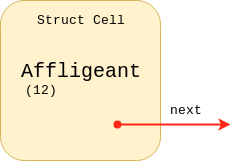
\includegraphics[scale=0.5]{structcell.png}
\caption{Structure d'une cellule}
\label{fig:structcell}
\end{figure}

Maintenant que nous savons comment modéliser un mot, il est important de souligner un point majeur de notre projet. Il nous est interdit de faire de l'allocation dynamique de mémoire. En effet, ce que nous utilisons sont des pointeurs vers des cellules. Afin de pouvoir créer des cellules à notre guise, il faut pouvoir les prendre quelque part : une \textit{piscine} de cellules.

Afin que l'on n'ait pas besoin d'utiliser des \inlinecode{C}{malloc} une \inlinecode{C}{struct pool pool} nous permet de \textbf{piocher dans des cellules \textit{free}} : à savoir de base $20000$ cellules disponibles.

\begin{lstlisting}
    struct pool {
        /* Tableau de cellules */
        struct cell m[MAX_CELLS];
        
        /* Pointeur vers la prochaine cellule libre */
        struct cell *next_free;
    };
\end{lstlisting}
\label{lst:struct_pool}

Lorsque l'on va créer une cellule, on va piocher dans celles qui ne sont pas utilisées : qu'elles soient à la suite ou pas, nous allons avoir soit :
\begin{itemize}
    \item une cellule libre
    \item \inlinecode{C}{NULL} si il n'y en a plus de libre
\end{itemize}

\begin{figure}[ht!]
\centering
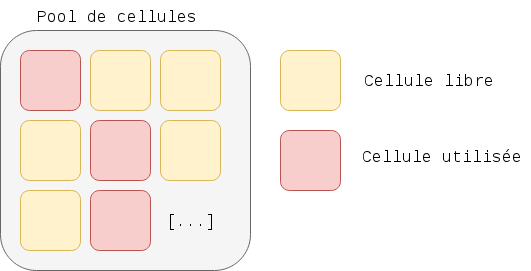
\includegraphics[scale=0.4]{pool.png}
\caption{Architecture de la \textit{pool} de cellules}
\label{fig:pool}
\end{figure}

La représentation sur ce schéma d'un grand carré (ressemblant à une piscine) n'est pas anodine. En effet, \textbf{les cases mémoires libres se trouvant n'importe où}, lorsque l'on va créer une nouvelle cellule, il n'est pas dit qu'elle se trouve à la fin de la \inlinecode{C}{pool} ou même à la suite de la dernière que nous venons de prendre.

Au final, la structure permettant de représenter les mots données par les consignes est totalement convenable et nous permet de bien représenter un texte.

% --- Files chaînées

\subsection{Files chaînées}
\label{subsct:file_chainee}

Cependant, nous avons d'une part une structure de données pouvant représenter les mots, mais nous devons toujours trouver comme les enregistrer et pouvoir y accéder. C'est donc pourquoi nous avons choisi d'implémenter un système de \textbf{liste chaînée à 2 entrées : une tête et une queue}.

Afin de pouvoir stocker les mots, les parcourir et les traiter nous avons fait le choix de créer une structure personnelle à savoir une file de cellules chaînées (d'où le nom file chaînée) :
\begin{lstlisting}
    struct queue {
        struct cell *first;
        struct cell *last;                                                     
        int cell_count;
    }; 
\end{lstlisting}
\label{lst:queue_base}

En effet, notre but étant de pouvoir lire un texte du début à la fin, de mémoriser ces mots dans cet ordre, et de pouvoir ensuite les ré-afficher dans le même ordre : cela correspond exactement à la définition d'une file :
\begin{itemize}
    \item \textbf{tête} : dans laquelle on va enfiler les mots qu'on lit un à un
    \item \textbf{queue} : mot que l'on va défiler afin de les afficher, ou bien tout simplement les traiter
\end{itemize}

Nous allons donc lire le fichier, et au fur et à mesure du parcours nous allons enregistrer les mots en les enfilant dans les files associées.

\begin{figure}[ht!]
\centering
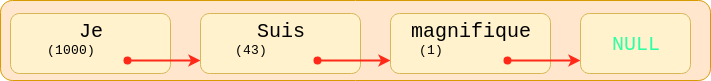
\includegraphics[scale=0.4]{structqueue.png}
\caption{Structure de file chaînée}
\label{fig:structqueue}
\end{figure}

Ce à quoi il faut faire attention durant l'élaboration de nos structures, c'est de prévoir une architecture propice à une complexité la plus basse possible selon nos usages de cette dernière. Dans la mesure où nous faisons \textbf{beaucoup d'ajouts et de retraits simples}, nous pouvons garder le principe d'une structure à deux extrémités.
La cellule \inlinecode{C}{*first} nous permet donc d'avoir accès à l'entrée de la file nous permettant d'enfiler les mots. Et de plus, la cellule \inlinecode{C}{*last} quant à elle nous permet de retirer les cellules.

Il est important de souligner \textbf{le fait qu'il s'agisse non pas simplement d'une file avec deux extrémités, mais une file chaînée}. En effet, le choix d'une file ne permet pas le parcours de cette dernière. Si l'on chaîne les éléments présents dans cette file, nous pouvons la parcourir et en ressortir des informations.

Le fait de prendre cette structure nous donne donc des \textbf{complexité concernant l'ajout et le retrait} en $\theta(1)$ cependant concernant le parcours de la file, il est en $\theta(n)$ avec $n$ le nombre d'éléments dans la file.

Il est vrai que nous aurions pu faire en sorte de prendre une autre structure afin de représenter les ensembles de mots : un tableau par exemple. Car en soi, il aurait seulement fallu garder en mémoire des indices de début de fin, comme cela nous pouvons effectuer : l'ajout, le retrait et l'accès à la case $i$ en $\theta(1)$. Cependant, vu qu'il s'agit d'une file de mots (une suite de mots) il était plus logique de partir sur ce principe et surtout plus simple (éviter de surcharger les structure d'informations trop lourdes).

% --- Singes

\subsection{Singes}
\label{subsct:singes}

Dans la version de base il existe plusieurs types de singes ayant chacun un travail à effectuer :

\begin{itemize}
    \item lecteur
    \item imprimeur
    \item statisticien
\end{itemize}

Nous avons mis un certain temps avant de structurer nos singes dans la mesure où nous souhaitions une \textbf{structure pouvant être adaptable à la suite des futures implémentations}.
En effet, le projet à pour but d'évoluer et afin de rendre la maintenance plus facile par la suite, il vaut mieux créer les structures intelligemment.

En ce qui concerne la modélisation des \inlinecode{C}{monkey} nous avons fait le choix d'utiliser une structure de données comme-ci contre :
\begin{lstlisting}
    struct monkey {
        enum role role;
        
        /* Sa file chainee associee */
        struct queue *queue;
        
        /* En greve ou non */
        int activity;     
    }; 
\end{lstlisting}
\label{lst:singes_conteneur}

\textbf{Partant du paradigme objet}, nous nous sommes dit qu'\textbf{il serait judicieux d'appliquer cette architecture} dans un projet en programmation impérative (choix que l'on contestera partie \ref{subsct:problemes} page \pageref{subsct:problemes}). Sur la page de présentation du projet, il était présenté du pseudo-code ressemblant à ceci : \inlinecode{C++}{selected_monkey.work()} \label{lst:work_method_poo}, ce qui nous a réconforté dans notre idée d'utiliser une structure représentant un singe.

Comme nous pouvons le voir, notre singe est donc doté d'un \inlinecode{C}{enum role role} à savoir un travail qu'il doit faire : \textit{lecture, statisticien, imprimeur}. Une énumération permet de lister les différents rôles que peuvent avoir un singe :
\begin{lstlisting}
/* Liste des roles */
    enum role {
        READER,
        STATISTICIAN,
        PRINTER,
        NB_TYPES
    }; 
\end{lstlisting}
\label{lst:enum_role}

Cette \inlinecode{C}{enum} nous permettra donc de pouvoir ajouter des futurs rôles dans les potentiels achievements qui arriveront. Chacun des singes aura donc un travail à effectuer selon une série de fonctions associées. Tout cela se gérera dans se fonction de travail \textit{work} :
\begin{lstlisting}
/* Fonction permettant de faire travailler un singe */
    int work(struct monkey *monkey,
            struct queue *queue,
            struct pool *pool);
\end{lstlisting}
\label{lst:code_work}

Nous venons donc de voir qu'un singe est une structure de données permettant de nous représenter une entité. Mais où les stocker ? Et comment savoir lequel est actif ou non ?

Pour ce faire, nous avons décidé d'utiliser \textbf{un tableau de pointeurs de singes} regroupant tous les singes du jeu :

\inlinecode{C}{struct monkey *monkeys[MAX_MONKEYS]}

Cette architecture nous permet donc d'avoir une liste de singes que nous pouvons manipuler à travers un tableau de structures de singes.

On pourra avoir accès à tous les singes grâce notamment à leur \inlinecode{C}{role} permettant donc d'\textbf{avoir accès directement à sa case dans le tableau}. Et par conséquent, nous il nous suffira d'appeler la fonction de travail en passant le singe en paramètre (qui possède sa file sur laquelle il travaille) sans se soucier de ce qu'il doit faire (cf. code précédent partie \ref{lst:code_work}).

Les \textbf{singes actifs} seront quant à eux manipulés dans \textbf{un autre tableau de pointeurs de singes actifs} : \inlinecode{C}{struct monkey *active_monkeys[MAX_MONKEYS]}\label{lst:active}. Il sera rempli à chaque tour en fonction de l'activité des singes.

% --- Singe lecteur

\subsubsection{Lecture du fichier : singe lecteur}
\label{subsct:reader}

Afin de récupérer notre fichier, il faut tout d'abord déléguer ce travail à quelqu'un : le singe lecteur. Pour cela nous avons tout simplement fait en sorte que le singe lecteur sache quel fichier il devait ouvrir à travers un pointeur de fichier \inlinecode{C}{FILE *fp} global. Ensuite, \textbf{à chaque mot que nous lisons, le singe doit l'ajouter dans la file du lecteur} (sa file). Le principe est très simple, à chaque mot qu'il lit, il l'ajoute et cela \textbf{remplit la file au fur et à mesure}.

\begin{figure}[ht!]
\centering
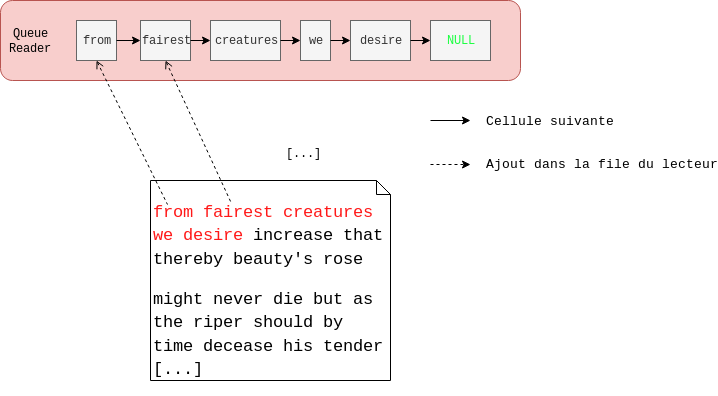
\includegraphics[scale=0.37]{schemacells.png}
\caption{Schéma de lecture du fichier}
\label{fig:schema_cells}
\end{figure}

Comme nous pouvons le voir sur la figure Figure \ref{fig:schema_cells}, au fur et à mesure que le singe lecteur travaille (et il reste toujours actif jusqu'à ce qu'il arrive à la fin du fichier), \textbf{il va lire les mots un par un}, \textbf{les remplir dans sa file} et \textbf{passer au mot suivant}. Cette file sera la base pour le travail du statisticien.

Comme nous l'avons expliqué auparavant, afin de pouvoir créer des cellules il devra piocher dans la piscine de cellules libre grâce notamment à la fonction :

\begin{lstlisting}
/* Fonction permettant de creer une nouvelle cellule */
    struct cell *create_new_cell(struct pool *pool,
                                    char word[],
                                    int noccs,
                                    struct cell *next);
\end{lstlisting}
\label{lst:code_create_new_cell}

A chaque nouveau mot lu, le singe lecteur va récupérer une cellule libre (qui vaudra \inlinecode{C}{NULL} si jamais il n'y a plus de place) et l'ajouter dans sa file par la biais d'une fonction :

\inlinecode{C}{int push(struct queue *queue,
                        struct cell *cell);}
\label{lst:push_explications}

Cette fonction va tout simplement \textbf{ajouter le mot dans la file}. L'architecture que nous avons choisi nous permet d'ajouter en temps constant $\theta(1)$ dans la file dans la mesure où nous avons accès à la première case.

Après avoir lu l'entièreté de son fichier, le singe se met en grève et ne se réveille pas.

% --- Singe statisticien

\subsubsection{Statistiques sur les mots : singe statisticien}
\label{subsct:statisticien}

Dans la version de base, le travail du statisticien consiste en \textbf{la lecture de la file du lecteur} et de \textbf{remplir la sienne mais de manière unique} (\textit{sans doublons}). Pour ce faire, il va lire la file du lecteur (qui va se vider par la suite : cf. partie \ref{subsct:printer} page \pageref{subsct:printer}).

\begin{figure}[ht!]
\centering
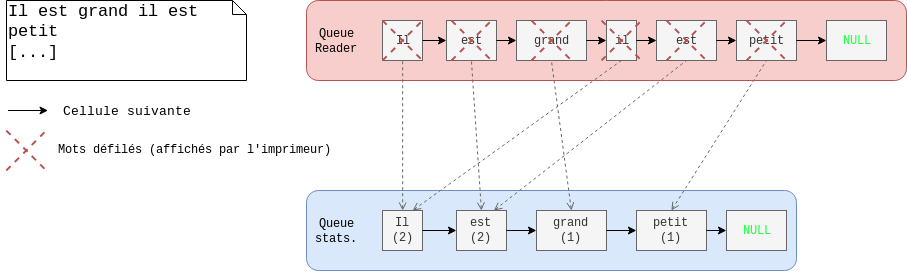
\includegraphics[scale=0.37]{schemastats.png}
\caption{Schéma des statistiques effectuées}
\label{fig:schema_stats}
\end{figure}

Le principe est donc simple : le lecteur va lire le fichier, et lorsque l'on ajoute un mot dans la file du lecteur alors le singe statisticien se remet en éveil (il change son état) et peut ensuite travailler.

Mais quel est au juste son travail ? Si la tête de la file du lecteur n'a pas été déjà lue par le statisticien et qu'elle n'est pas vide : il remplit sa file (cf. Figure \ref{fig:schema_stats}). \textbf{Sa file a un comportement différent de celle du lecteur}. En effet, elle fait \textbf{apparaître seulement les mots de manière unique}, à savoir que dans cette file, \textbf{le nombre d'occurrences sera important}. Quand on va ajouter une cellule dans sa file, le statisticien prendra soin de \textbf{vérifier si une cellule existe déjà ou pas}, et donc si un mot a déjà été lu.

Pour effectuer son travail, une fonction lui est attribuée :
\begin{lstlisting}
/* Liste des roles */
    int stats(struct monkey *monkey,
              struct queue *queue,
              struct pool pool) 
\end{lstlisting}

En utilisant une fonction \textbf{différente} de celle qu'utilise le lecteur, la fonction de travail du statisticien va appeler une fonction permettant d'ajouter une cellule avec un comportement différent (sans les doublons) :

\begin{lstlisting}
/* Push sans doublon */
    int push_uniq(struct queue *queue,
                    struct cell *cell);
\end{lstlisting}
\label{lst:push_uniq_explications}

Cette fonction est légèrement différente de celle précédente, à ceci près qu'elle utilise une fonction auxiliaire très intéressante et essentielle quant à la fonction du singe statisticien :

\inlinecode{C}{check(struct queue *queue, struct cell *c)}
\label{lst:check_explications}

Cette fonction va nous \textbf{renvoyer un pointeur vers la cellule si cette dernière existe dans la file}, et \inlinecode{C}{NULL} sinon. Cette fonction a une complexité $\theta(n)$. En effet, le statisticien parcourt la liste des mots qui ont déjà été lus. Donc supposons qu'à chaque appel de la fonction le statisticien parcourt sa liste de mots, la complexité est très vite élevée cependant notre architecture logicielle concernant les files chaînées ne nous permet pas d'avoir une complexité plus faible. Si nous avions pu utiliser les \inlinecode{C++}{std::map} (analogue en C++) nous aurions pu grandement réduire la complexité quant au parcours des mots, cependant elle n'aurait pas été optimale concernant l'ajout et retrait des mots depuis les files.

Nous aurions pu nous dire de trier les mots par ordre lexicographique afin de pouvoir par la suite effectuer une recherche dichotomique en $\theta(n.\log(n))$. Malgré le fait que l'ordre dans lequel les mots apparaissent dans la file, il ne s'agit pas d'un tableau avec lequel nous pouvons avoir accès à la case $i$ en $\theta(1)$ et donc il est inutile de le trier dans la mesure où si l'on souhaite avoir accès à la case $k$ nous devons parcourir toutes les cases allant de 1 à $k$.

L'avantage majeur est que cette fonction va vérifier s'il existe déjà la case que le statisticien lit dans sa file associée, cela entraîne ainsi \textbf{une économie de cases mémoires}. Si un texte contient $20000$ fois le même mot, au lieu d'avoir une file de $20000$ cases, nous aurons une file d'un seul mot ayant pour nombre d'occurrences $20000$ (et la complexité de la fonction \inlinecode{C}{check} aura certes une complexité de $\theta(n)$ mais avec un $n$ peu élevé). C'est donc pourquoi nous avons fait le choix de garder cette complexité à défaut de ne pas pouvoir la réduire.

Par la suite si le mot n'existe pas, il le rajoute dans la file (en utilisant la fonction \inlinecode{C}{push} du singe lecteur), sinon augmente juste son nombre d'occurrences.

Ce singe quant à lui se met en grève seulement \textbf{s'il a déjà lu le premier mot de la file ou bien si la file du lecteur est vide}. Si ce n'est pas le cas, il se remettra actif et pourra donc continuer de travailler (nous allons aborder cette partie page \pageref{subsct:boucle_jeu} partie \ref{subsct:boucle_jeu}).

% --- Singe imprimeur

\subsubsection{File du lecteur se vide : singe imprimeur}
\label{subsct:printer}

Le singe lecteur quant à lui, travaille si et seulement si le premier mot a été lu par le statisticien. Si oui, son but va être alors d'imprimer le mot et de l'enlever de la file. Lorsqu'il va retirer les mots de la file, la fonction \inlinecode{C}{pop(struct queue *queue)} \label{lst:pop_explications} va \textbf{enlever la cellule que nous venons d'imprimer}. En effet, nous aurions pu faire en sorte de la laisser dans la file pour un futur usage, cependant, en terme de complexité pour les parcours cela aurait été beaucoup plus élevé.

Supposons que nous n'enlevions pas la cellule, alors nous aurions du parcourir la file du statisticien à la recherche de la première cellule qui n'a pas été imprimé : $\theta(n)$ à chaque impression de mot. Dans la mesure où notre complexité est déjà élevée concernant la recherche d'un mot.

De plus, cette fonction \inlinecode{C}{pop} n'aura pas pour effet seulement de se repérer quant aux mots déjà imprimés par l'imprimeur. En effet, vu que ce singe va modifier la file de mots du lecteur, le statisticien lui aussi n'aura pas besoin d'effectuer des recherches supplémentaires quant au premier mot qu'il n'a pas ajouté dans sa file. Par conséquent cela nous permet aussi d'éviter une complexité $\theta(n)$ pour la recherche de la première cellule du statisticien.

\begin{figure}[ht!]
\centering
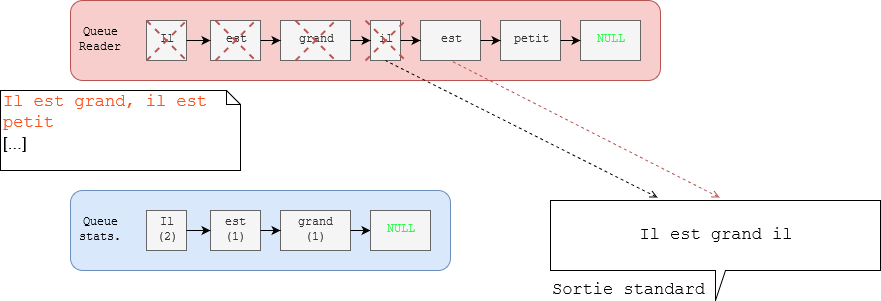
\includegraphics[scale=0.5]{schemaimprimeur.png}
\caption{Schéma de l'impression sur la sortie standard}
\label{fig:schema_imprimeur}
\end{figure}

% --- Utils

\subsection{Utils}
\label{subsct:utils}

Ces fichiers servent seulement à pouvoir avoir accès à différentes fonctions utiles, à savoir :
\begin{itemize}
    \item récupération de la seed
    \item afficher l'usage lorsque ce dernier n'est pas bon
    \item renvoyer un nombre aléatoire
\end{itemize}

Outre le fait de nous donner des fonctions utiles (d'où le nom...) ces fichiers n'ont que très peu d'utilité et il est inutile de s'attarder dessus.

% --- Makefile

\subsection{Makefile}
\label{subsct:makefile}
Dans notre architecture, un fichier occupe une place très importante : il s'agit du \textit{Makefile}. En effet, afin d'éviter de recompiler tous les fichiers à la main, nous avons créer ce fichier permettant d'automatiser tout le processus de compilation.

Pour ce faire nous avons écrit différentes règles ; permettant de nettoyer le projet, compiler toutes les dépendances et effectuer les tests.

Concernant le nettoyage du code, rien de plus simple : il suffit de nettoyer tous les fichiers objets du dossier dans lequel on souhaite compiler mais aussi dans le dossier test, à l'aide de la règle \textit{clean}. En effet, ces fichiers ne sont pas utiles dans la mesure où l'on va les régénérer lors de la compilation de notre programme.

Maintenant concernant notre compilation, notre règle par défaut \textit{all} a pour but de compiler chacune des dépendances dans le bonne ordre pour ensuite générer l'exécutable du \textit{main}. Cette dernière appelle une règle \textit{code} qui elle-même appelle une règle \textit{code-achiev1}. Cela a été réalisé dans l'hypothèse où d'autres dépendances devraient s'ajouter ou bien si plusieurs versions du projet venaient à devoir co-exister dans la même arborescence.  À noter que nous n'avons qu'un \textit{Makefile} par version (sauf celui des tests) dans la mesure où les autres sont dans les autres branches de notre Git.

Concernant les règles du \textit{Makefile} nous utilisons des variables nous permettant d'alléger le code. Parmi celles-ci :
\begin{itemize}
    \item \$@ : permet de connaître la cible concernée
    \item \$\textless : permet d'avoir accès au premier composant de la règle (notamment utile pour l'option -c avec la compilation sous \textit{gcc})
    \item \$\textasciicircum : permet d'avoir accès à tous les composants d'une règle 
\end{itemize}

Ces différentes variables vont nous permettre de générer tout le code dont nous avons besoin de manière automtisée sans avoir à marquer chacune des lignes de code. Le tout de la manière la plus factorisée possible ! De plus, d'autres variables concernent l'ensemble des dépendances (notamment les fichiers que nous avons besoin pour les dépendances ou bien le compilateur que nous utilisons par défaut et ses flags).

Le même principe est appliqué concernant les tests. Il suffit de lancer le \textit{Makefile} avec comme règle : \textit{test} et la compilation et le lancement des tests s'effectuera. Il va se déplacer dans le dossier des tests et effectuer l'ensemble des règles à l'intérieur. Chaque fichier test sera compilé et lancer (un fichier test par notion : sur les cellules, les files, les singes, etc...).

Enfin, les règles \textit{report} et \textit{view} permettent respectivement de compiler le fichier rapport .tex en pdf à l'aide de \textit{pdflatex} ainsi que de lancer la visionneuse de documents PDF \textit{evince} sur ce fichier.

% --- Tests, input et rapport

\subsection{Tests, input et rapport}
\label{subsct;test_input}

Nous avons intégré différents dossiers dans l'architecture de notre projet concernant les \path{tests/}, les données \path{input/} et le rapport que nous livrerons avec la version non compilée \path{
rapport/}.

Commençons par les \path{input/}. Il servent tout simplement de base au projet. Ils constituent un jeu de données remplissant la plupart des cas relatifs au projet : long texte, court texte, texte vide...

Quant au rapport, rien de bien intéressant. Il s'agit d'un dossier contenant tous fichiers concernant le rapport. Il a été écrit sur la plateforme collaborative \textit{Overleaf} et a bien été testé sur machine \textbf{\textit{pedago}} avant rendu.

 \textbf{Attention}, afin de pouvoir compiler le rapport, il faudra vérifier que le paquet \textit{algorithm2e} est présent. Nous l'avons ajouter au dossier du rapport. Il est donc nécessaire de compiler dans le dossier afin de ne pas générer d'erreurs.

Maintenant venons-en à la partie la plus intéressante : les tests. Il était vital d'effectuer des tests afin d'être sûr d'obtenir du code fonctionnel et solide. Pour ce faire, nous avons décidé d'écrire des fichiers tests pour chaque ensemble de fonctions agissant sur des mêmes structures. Par exemple, nous avons écrit des tests concernant les entrées-sorties, des tests sur les files, d'autres sur le travail des singes (un par singe). L'utilité est de rassembler les principales fonctions agissant sur le programme en un seul fichier.

Le \textit{Makefile} (cf. partie \ref{subsct:makefile} page \pageref{subsct:makefile}) va nous compiler l'entièreté des programmes et les lancer. Nous saurons donc si les tests ont échoué ou non. Ils testent par exemple, si une file est bien vide, si on ajoute bien une cellule dans une file lorsque le lecteur lit, si les statistiques sont bien effectuées ou même si l'écrivain (que l'on verra après, partie \ref{subsct:ecrivain} page \pageref{subsct:ecrivain}) choisit bien des mots aléatoirement ! La plupart de ces tests se basent sur un jeu de test indépendant, contenu dans le fichier \path{tests/input.txt}, notamment pour les tests des différents singes et de la file.

Ces tests sont donc la pierre angulaire de notre projet nous permettant de savoir ou non si lorsque l'on effectue un changement dans le code, nous avons cassé quelque chose !

% ------------------ Jeu --------------------

\section{Jeu}
\label{sct:jeu}

% --- Compilation et lancement du programme

\subsection{Compilation et lancement du programme}
\label{subsct:compilation}

Maintenant que nous avons toutes nos structures et l'intégralité de notre architecture logicielle, nous pouvons modéliser un exemple type de partie allant de la compilation du programme, en passant par les différents tours de jeu jusqu'à l' \textit{output} final de la version de base.

Avant toute chose afin de pouvoir compiler le programme il faudra faire en sorte d'utiliser les commandes du \textbf{Makefile} (détaillées partie \ref{subsct:makefile} page \pageref{subsct:makefile}). Il faudra donc nettoyer le projet (essentiellement les fichiers \path{.o}) et complier toutes les dépendances. Après cela vous pourrez lancer le programme.

Pour ce faire, il suffit de rentrer cette ligne de commande dans le dossier du programme :

\inlinecode{bash}{./project file -s seed -t numberturns}
\label{lst:bash_line}

La commande est semblable qu'importe la version du projet (cependant, la version de base présente dans la branche \textit{base} du Git ne contient pas l'option \textit{- t}). L'ordre des arguments n'est pas restreint, il suffit seulement de notifier les chiffres relatifs aux options \textbf{directement} après les options relatives.

Vous pouvez piocher dans le dossier du jeu de données \path{input/} afin de ne pas à avoir des fichiers à créer.

% --- Boucle de jeu

\subsection{Boucle de jeu}
\label{subsct:boucle_jeu}

Maintenant que nous connaissons les missions principales de chacun des singes, il est désormais temps de simuler une partie de jeu afin de savoir comment interagissent entre eux les singes.

\begin{algorithm}[H]
$queues \gets init\_queues()$\;
$monkeys \gets init\_monkeys()$\;

 \While{at least one monkey active AND not enough turns played}{
  $active\_monkeys \gets filter\_active\_monkeys(monkeys)$\;
  $random\_monkey \gets select\_random\_monkey(active\_monkeys)$\;
  
  $work(random\_monkey,queues)$\;
  $check\_activities(monkeys,queues)$\;
 }
$display\_stats()$\;
\caption{Boucle de jeu}
\end{algorithm}
\label{algo:game}

La boucle de jeu de la version de base est très simple. Au début du lancement du programme, nous allons \textbf{initialiser tout ce dont nous avons besoin} : que cela soit les files, les singes ou mêmes l'entièreté des variables simples.

Ensuite il suffit de lancer le jeu : ce dernier \textbf{se termine} lorsque soit :
\begin{itemize}
    \item le nombre de tours à été dépassé
    \item tous les singes sont en grève
\end{itemize}

Et donc à chaque tour de jeu nous allons \textbf{filtrer tous les singes actifs et en sélectionner un} parmi ces derniers. Que cela soit un singe lecteur, statisticien ou imprimeur, nous n'allons pas différencier sa fonction de travail dans la boucle de jeu principal car au final ils font tous la même chose : ils travaillent. Nous l'avons détaillé précédemment (partie \ref{lst:code_work} page \pageref{lst:code_work}) mais c'est dans la fonction de travail que nous allons choisir le travail à effectuer selon le rôle du singe.

À partir de cette étape, les singes vont donc \textbf{interagir avec le fichier} et au fur et à mesure le jeu va avancer. Nous avons rajouter une fonction \textit{check\_activities} qui permet de \textbf{s'assurer si nous pouvons réactiver des singes} : notamment selon leurs modalités de travail (cf. partie \ref{subsct:statisticien} page \pageref{subsct:statisticien}). Et nous allons répéter ces tours de jeu.

Prenons un scénario avec seulement un fichier de quatre mots : \textit{Bonjour je suis je}. Le \textbf{lecteur va lire le premier mot du texte}. Cette action aura pour effet de réveiller le \textbf{singe statisticien qui pourra l'ajouter à sa file}. Après l'avoir fait, le \textbf{singe imprimeur pourra l'afficher et le retirer de la file}.
Ce système va se répéter au fur et à mesure afin de générer des données comme celles-ci à la fin (les singes rouges sont inactifs et les mots rouges sont lus par le lecteur ou le statisticien) :

\begin{figure}[ht!]
\centering
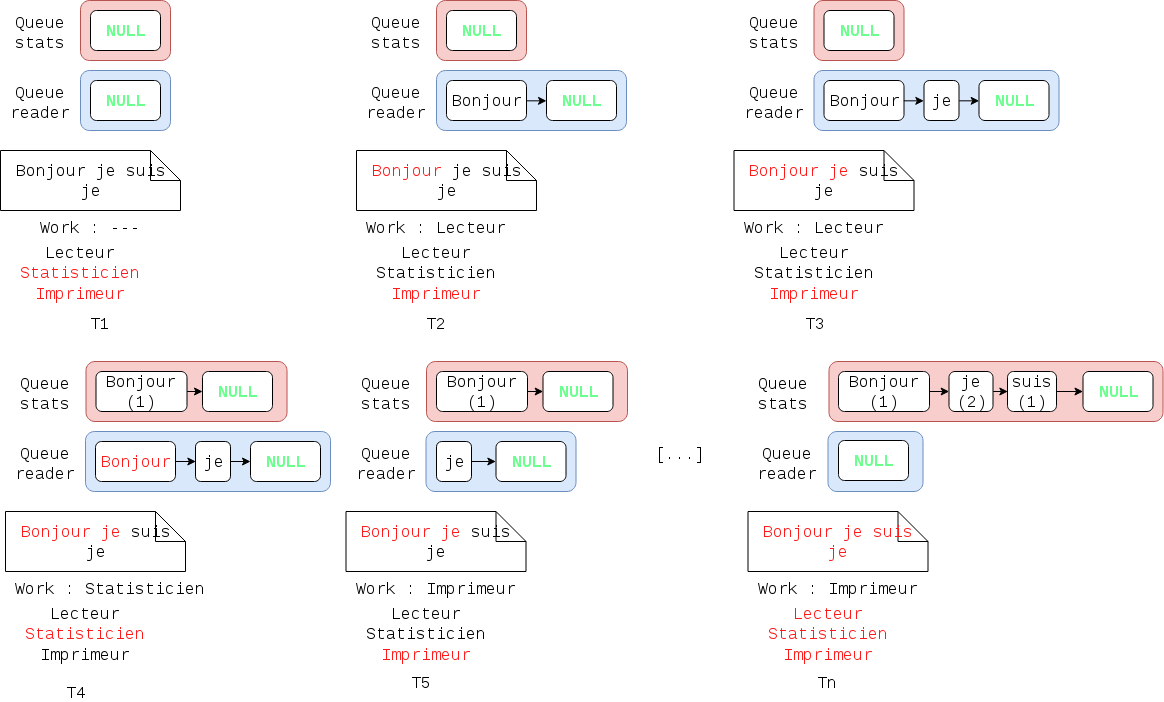
\includegraphics[scale=0.35]{game.png}
\caption{Schéma d'une boucle de jeu possible}
\label{fig:game}
\end{figure}

Bien sûr, il s'agit d'une boucle potentielle de jeu. Dans la mesure où la notion d'aléatoire intervient, pour peu que le nombre de tours suffise, le résultat sera le même mais pas l'ordre dans lequel il s'effectue.

% --- Output final

\subsection{\textit{Output} final}
\label{subsct:output_final}

L'affichage dans le terminal, concernant la base version, sera semblable à celui ci (tout dépend de la quantité de mots lus mais aussi le nombre de tours joués).

\begin{figure}[ht!]
\centering
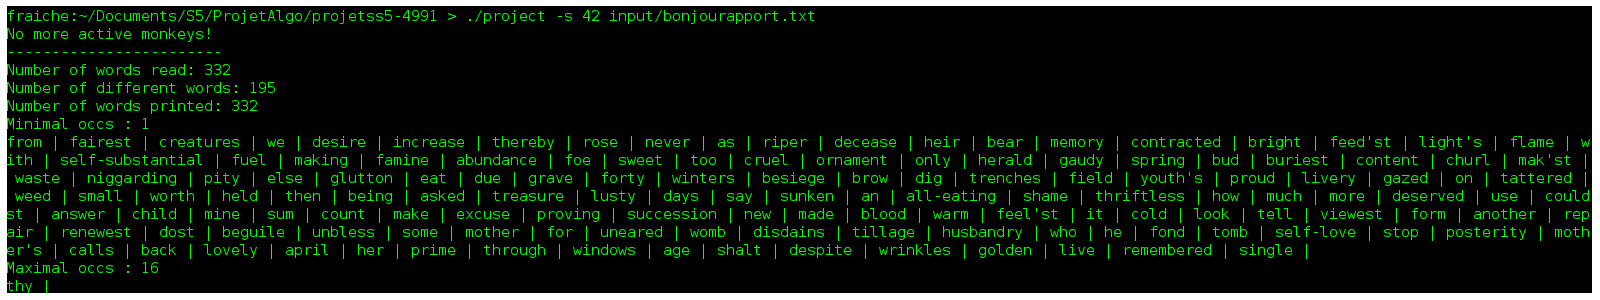
\includegraphics[scale=0.29]{output.png}
\caption{Exemple d'une sortie finale sur la sortie standard}
\label{fig:output}
\end{figure}

On peut voir la condition d'arrêt du jeu, mais aussi des statistiques concernant les mots lus, comptés, etc... Et enfin les mots concernant les occurrences maximales et minimales.

% ------------------------ Achievement 1 -------------------------

\newpage
\section{Achievement 1}
\label{sct:achiev1}

Après avoir terminé la version de base dans les temps, nous avons pu commencer l'achievement numéro 1. Il y a beaucoup de choses qui se différencient de la version de base. En effet contrairement à l'ancienne version dans laquelle le singe statisticien se contentait d'effectuer des statistiques sur les mots en les stockant dans sa structure et l'imprimeur quant à lui, affichait les mots sur la sortie standard. Dorénavant ils devront ne plus se contenter de cela.

En effet, un autre singe est désormais de la partie : le singe \textbf{écrivain}. Ce singe aura pour rôle de \textbf{produire des mots} : à savoir \textbf{écrire des phrases depuis le texte déjà existant}. Pour ce faire, l'architecture de notre projet devra changer. Ce nouveau singe devra donc choisir un mot depuis ceux déjà lus par le statisticien, et construire des phrases.

% --- Mots successeurs
\subsection{Mots successeurs}
\label{subsct:mot_successeurs}

Afin de pouvoir récupérer les mots depuis ceux déjà lus par le statisticien, l'écrivain devra donc y avoir accès. Sa mission principale est de reproduire des morceaux de phrases existants et les réécrire. Pour ce faire nous avons choisi d'ajouter une nouvelle variables dans les cellules, à savoir : \textbf{une file chaînée de successeurs} :
\begin{lstlisting}
/* Nouvelle implementation de cell */
    struct cell {
        char word[MAX_WORD_LENGTH+1];  
        int  noccs;              
        struct cell* next;
        
        /* Liste de mots successeurs */
        struct queue *queue;
    };
\end{lstlisting}
\label{lst:nouvelle_impl_cells}

Il était nécessaire d'enrichir cette structure dans la mesure où nous ne pouvions pas faire ce qui était demandé avec le peu d'informations que l'on avait.

Nous avons donc fait le choix d'ajouter un champ \inlinecode{C}{*queue} dans la structure des cellules. Le but étant de rajouter des mots successeurs à ce que l'on a lu afin de pouvoir réécrire des phrases. Avec cette implémentation, lorsque le \textit{statisticien} lira un mot, il prendra soin de vérifier que le mot qu'il lit (cf. Figure \ref{fig:successors_schema}):
\begin{itemize}
    \item possède un suivant : l'ajoute donc dans sa file des successeurs
    \item ne possède pas de suivant :
    \begin{itemize}
        \item \textbf{lecteur n'a pas fini de lire} (forcément des mots le suivent) : se remet en grève pour attendre
        \item \textbf{lecteur a fini de lire} : alors considère qu'il a lu le mot 
    \end{itemize}
\end{itemize}

Mais cela veut dire que lorsque l'on crée une cellule et que l'on souhaite la manipuler, il faut que tous ses champs existent. Pour cela, le champ \inlinecode{C}{*queue} doit exister. Afin de pouvoir créer des files dans les cellules de manière dynamique nous avons donc fait (à l'image de ce qui nous avait été donné pour les cellules) une fonction qui a pioché dans une \textit{piscine} de files :

\begin{lstlisting}
/* Implementation de la \textit{pool} de files */
    struct poolQueues {
        struct queue m[MAX_QUEUES];
        struct queue *next_free;
    };
 
/* Fonction permettant de creer des files */
struct queue *create_new_queue(struct poolQueues *poolQueues,
                                struct cell *first,
                                struct cell *last);
\end{lstlisting}
\label{lst:create_new_queue}

Lorsque l'on va appeler la fonction permettant de créer de nouvelles cellules, alors on piochera aussi dans une \textit{piscine} de files afin d'en avoir. Nous avons choisi cette implémentation dans la mesure où avec une \inlinecode{C}{poolQueues} nous pouvons \textbf{restreindre la quantité de files allouées} (à la même hauteur que celle des cellules).

\begin{figure}[ht!]
\centering
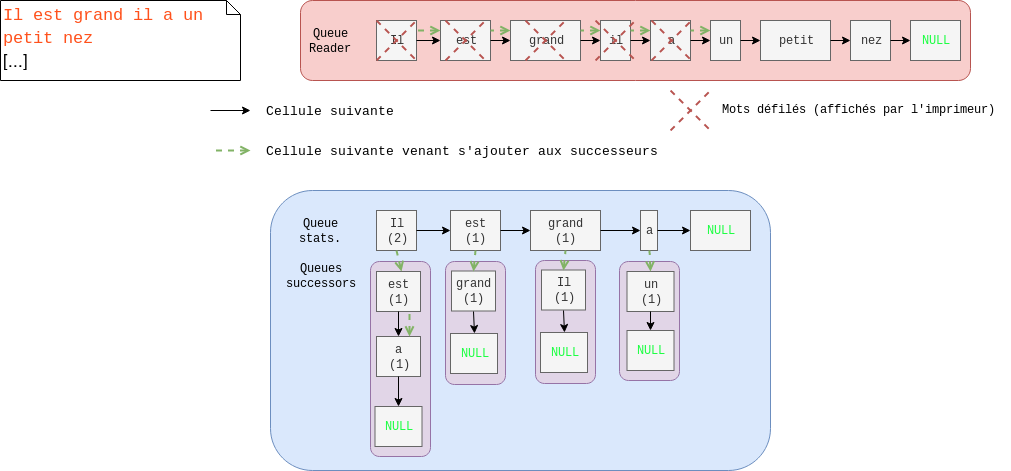
\includegraphics[scale=0.35]{successorsschema.png}
\caption{Schéma de l'ajout des cellules suivantes dans la file du statisticien}
\label{fig:successors_schema}
\end{figure}

Nous avons pris l'exemple d'une situation dans laquelle le texte n'a pas fini d'être lu. Lorsque le statisticien lira un mot, il ajoutera le suivant (s'il existe) dans sa file de successeurs. Grâce à cela, nous aurons une suite de mots dans lesquels nous pourrons piocher.

Ce système nous permet donc de faire en sorte qu'à chaque tour de jeu, lorsque le statisticien se met à travailler, il va \textbf{ajouter au fur et à mesure les successeurs dans sa structure dédiée}. Et cela ne change pas du tout que le mot existe déjà ou pas dans la file du statisticien. En effet, comme nous l'avons dit précédemment, une fonction \inlinecode{C}{check} nous permet de potentiellement récupérer une cellule déjà présente dans la file du statisticien. Et comme la fonction \inlinecode{C}{check} nous \textbf{renvoie} un pointeur vers cette cellule, nous avons juste à la manipuler et le tour est joué.

\label{complexite_successors}

La complexité concernant l'ajout dans la file des successeurs \textbf{n'est pas différente de celle d'un ajout dans la file du statisticien} (et elle s'effectue juste après cette dernière d'ailleurs) dans la mesure où nous vérifions si un mot existe déjà dans les successeurs. Nous aurions pu faire en sorte de l'ajouter de manière arbitraire à la fin de la file sans compter les multiplicités. Cela aurait fait en sorte de réduire la complexité de $\theta(n)$ à $\theta(1)$.

Cependant, nous avons fait le choix de \textbf{garder la file des successeurs comme celle du statisticien}, à savoir : \textbf{une file ne possédant pas de doublons} afin de pouvoir économiser beaucoup de mémoire allouée. Supposons qu'un texte contiennent beaucoup de doublons (voyons grand, des milliers !), avec notre architecture qui consiste à enlever les doublons, on fera en sorte que :
\begin{itemize}
    \item file statisticien : très peu de cellules (car beaucoup de doublons)
    \item file successeurs : très peu de cellules (pareil)
\end{itemize}

Le tour est joué car il nous suffit ensuite, après vérification si la cellule lue existe dans la file des mots du statisticien, de remplir la file de la cellule avec le mot qui suit :

\inlinecode{C}{push_uniq(monkey->queue,copy);}

Cela veut dire tout simplement que l'on ajoute de manière unique (cf. partie \ref{lst:push_uniq_explications} page \pageref{lst:push_uniq_explications}) dans la file afin d'avoir la liste des successeurs d'un mot.

% --- Écrivain

\subsection{Nouveau singe : l'écrivain}
\label{subsct:ecrivain}

Désormais il existe un nouveau singe : le singe écrivain. Ce dernier a pour mission de reproduire des bouts de phrases existants. Comme nous venons d'implémenter les mots successeurs dans la file de cellules elles mêmes, il suffisait donc de piocher dans la file du statisticien et de reproduire des phrases vu que nous possédons tous les successeurs. L'écrivain va donc :
\begin{enumerate}
    \item \textbf{tirer un mot aléatoirement} depuis la file du statisticien
    \item \textbf{le garder en mémoire} (important)
    \item se mettre potentiellement en grève
    \item \textbf{écrire ce mot} et \textbf{en choisir un autre}
    \item terminer ses phrases par de la ponctuation
\end{enumerate}

Cette boucle de travail est à refaire indéfiniment : le singe écrivain ne se met jamais en grève.

Le rôle de l'écrivain est donc de piocher depuis la file du statisticien des mots de manière aléatoire afin de reproduire des phrases. \textbf{Il reste en grève durant les 100 premiers tours} dans la mesure où si nous le faisions travailler directement, il n'aurait pas beaucoup de mots à lire possédant de suivants vu que le statisticien n'a pas encore forcément eu le temps de lire beaucoup de mots.

Mais un problème survient : où peut-on stocker le mot que le singe choisi aléatoirement et où peut-on remplir les phrases? (qui seront lues par l'imprimeur que l'on verra juste après partie \ref{imprimeur_achiev1} page \pageref{imprimeur_achiev1}) C'est donc pourquoi nous avons aussi choisi de \textbf{modifier la structure de singes} :
\begin{lstlisting}
/* Nouvelle implementation des singes */
    struct monkey {
        enum role role;
        struct queue *queue;
        int activity;
        
        /* Possede sa cellule */
        struct cell *cell;
    }; 
\end{lstlisting}
\label{lst:nouvelle_impl_singe}

Grâce à ce nouveau champ on peut choisir une cellule aléatoirement, l'ajouter dans le champ et depuis ce champ récupérer les successeurs et en reprendre un aléatoirement.

Pour ce faire, nous avons créer deux fonctions afin de choisir des mots aléatoirement :

\inlinecode{C}{monkey->cell = random_cell(queueStats);}

\inlinecode{C}{struct cell *random = random_cell_with_occs(monkey->cell->queue);}.
\label{lst:random_cells}

\label{complexite_random_cell}

Ces deux fonctions ont une utilité semblable mais sont différentes en terme de complexité. En effet, la première choisit une cellule aléatoirement dans une file (en l'occurrence dans la file du statisticien) et la renvoie : complexité $\theta(n)$ dans le pire des cas. Elle se contente de choisir une cellule au hasard entre la première et la dernière.

En revanche, la deuxième fonction est différente. Elle prend en compte le nombre d'occurrences dans la file. Supposons que l'on possède une file de mots avec 1000 fois le mot \textit{the}, et une seule fois le mot \textit{Sup'eirb} alors on aura beaucoup plus de chances de tomber sur le premier mot (c'est pas faute d'avoir essayé !). Et donc cette fois-ci il faut déjà parcourir la file afin de connaître la somme des occurrences de tous les mots présents à l'intérieur et ensuite aller chercher le mot, soit une complexité de : $\theta(2n)$.

Ci-contre un schéma représentant la construction d'une phrase aléatoirement grâce à la file du statisticien :

\begin{figure}[ht!]
\centering
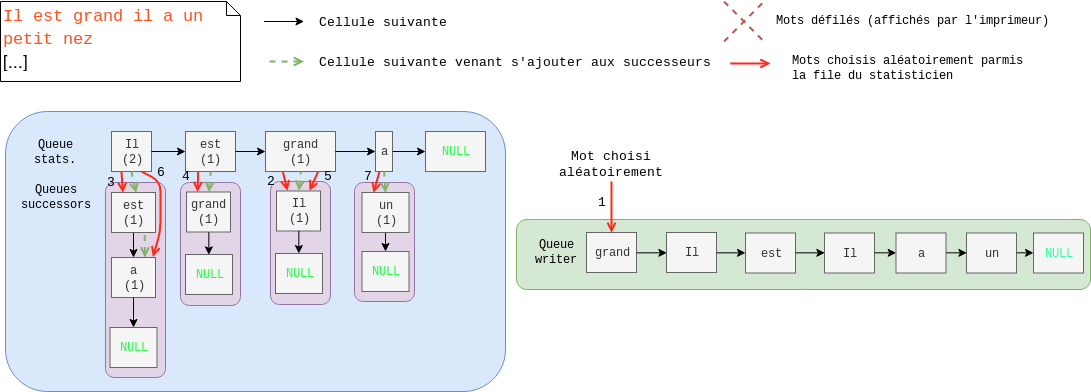
\includegraphics[scale=0.35]{writerwork.png}
\caption{Exemple de création de phrases}
\label{fig:writer_work}
\end{figure}

Nous pouvons voir (dans l'ordre des numéros) que l'\textit{écrivain} va choisir aléatoirement dans la file du statisticien afin d'enfiler dans sa \inlinecode{C}{*queue} . Grâce à l'architecture, l'\textit{écrivain} va donc pouvoir recréer des bouts de phrases déjà existantes.

Nous aurions pu faire en sorte que la complexité des fonctions baissent notamment en passant les structures sous forme de tableau : dans laquelle la complexité pour récupérer un élément à un emplacement est constante, mais cela aurait beaucoup plus pénalisé le reste du projet et dans la mesure où nous étions parti avec l'idée de garder nos files, il était nécessaire de ne pas y toucher.

% --- Nouveaux rôles

\subsection{Nouveaux rôles}
\label{subsct:nouveaux_roles}

\label{imprimeur_achiev1}
Dans la version de base, le rôle de l'imprimeur était d'afficher sur la sortie standard les mots que le statisticien venait de lire (il se mettait actif dès qu'un mot était lu par ce dernier). Désormais ce n'est plus le cas. En effet, il se met actif lorsque la file de l'écrivain est remplie. Dans la mesure où l'écrivain reste inactif les 100 premiers tours afin qu'il puisse avoir un ensemble déjà conséquent de mots, \textbf{l'imprimeur est donc lui aussi en grève au départ du jeu}. Dans la figure ci-dessus (cf. partie \ref{fig:writer_work} page \pageref{fig:writer_work}) il va \textbf{reproduire son ancien travail mais sur une file } : il devra retirer une à une les cellules de la file de l'écrivain et les afficher.

\label{stats_achiev1}
C'est donc là que notre implémentation est intelligente et pratique, elle permet lors de l'initialisation des singes d'associer la file de l'écrivain à celle de l'imprimeur :

\inlinecode{C}{struct monkey printer = {2,0,&queueWriter,NULL}}
\label{lst:printer_init}

Grâce à cela, il devra seulement avoir accès à sa file et donc la lire et la défiler. Mise à part cela, l'imprimeur, dans cet achievement, ne comporte pas d'autre changement. En effet, son rôle est le même en miroir avec celui de la première version.

Quant au statisticien, il n'a donc plus seulement le rôle d'effectuer des statistiques mais il doit aussi \textbf{retirer les cellules au fur et à mesure de la lecture dans la file des mots}.

% --- Nouvel output

\subsection{Nouvel \textit{output}}
\label{subsct:nouvel_output}

Maintenant que notre jeu a un peu évolué, le résultat final est par conséquent différent. Maintenant nous avons un texte produit aléatoirement qui est affiché. Voici un exemple de sortie que nous avons après avoir fait tourné notre programme avec un court texte :

\begin{figure}[ht!]
\centering
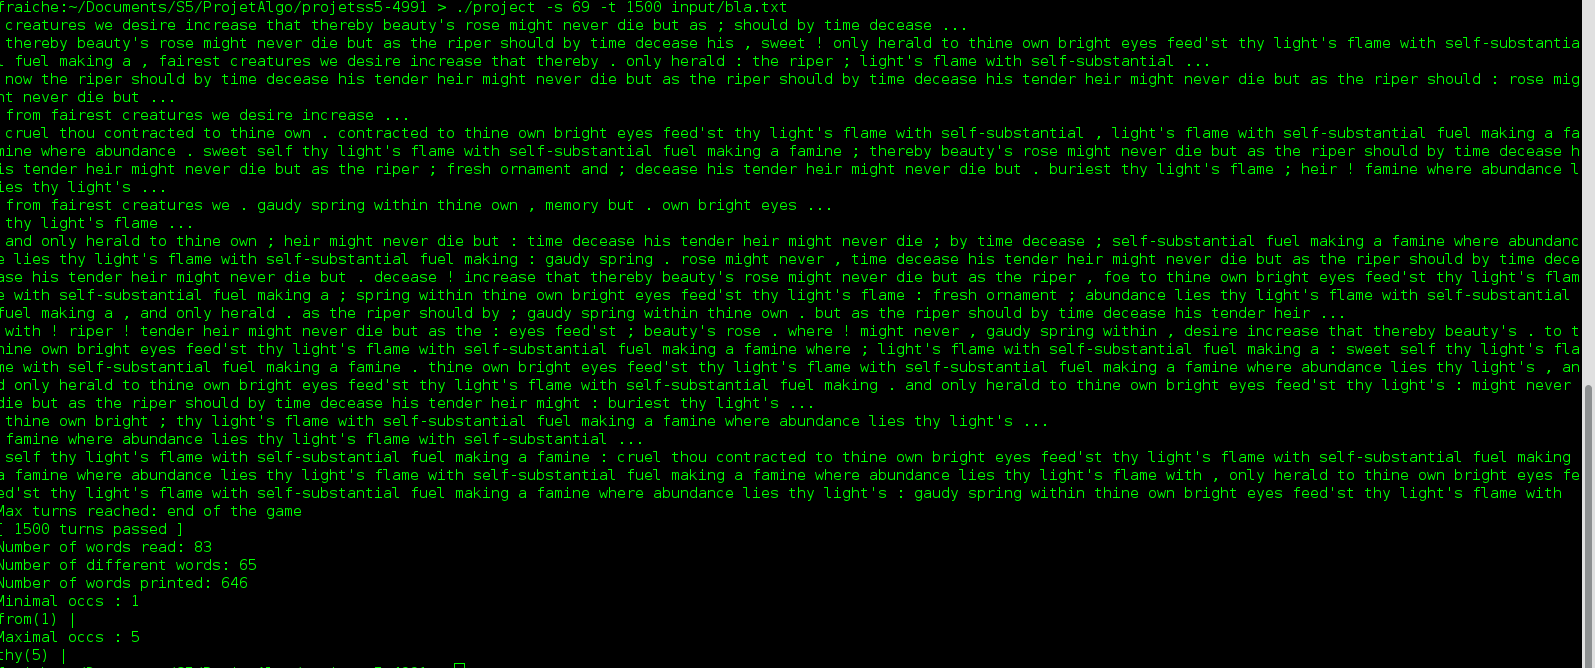
\includegraphics[scale=0.28]{outputachiev1.png}
\caption{Exemple d'une sortie finale sur la sortie standard pour l'achievement 1}
\label{fig:output_achiev1}
\end{figure}

On peut maintenant voir les phrases qui ont été produites par l'écrivain et affichées par l'imprimeur.


% ------------------ Capitalisation d'expérience --------------------

\newpage
\section{Capitalisation d'expérience}
\label{sct:capitalisation}

% --- Problèmes

\subsection{Problèmes rencontrés}
\label{subsct:problemes}

% --- Mauvaise architecture des singes

\subsubsection{Mauvaise architecture des singes}
\label{subsct:mauvaise_archi_singes}

Il est important de bien détailler l'un de nos principaux problèmes. En effet, comme nous l'avons indiqué partie \ref{lst:singes_conteneur} en page \pageref{lst:singes_conteneur}, nous avons fait le choix d'utiliser un tableau de pointeurs de singes (qui sont eux-mêmes des structures de données). Cependant... cela est totalement foireux ! En effet, voulant partir d'une bonne intention en adoptant une architecture ressemblant à celle de l'orienté objet, nous nous sommes rendu compte qu'il n'était pas du tout optimisé.

En effet, nous aurions pu tout simplement utiliser un tableau d'entiers afin de savoir si les singes sont actifs ou non (pour la version de base). Ou bien utiliser un tableau de singes et non pas un tableau de pointeurs de singes (ce qui change la donne !) :

\inlinecode{C}{struct monkey monkey[MAX_MONKEYS]}

Ceci à la limite aurait été plus intelligent dans la mesure où nous aurions pu initialiser le tableau de singes dans une fonction de manière propre, et pas dans le \inlinecode{C}{main} de manière peu conventionnelle.

De plus, nous pensons que si nous avions adopté un conteneur de singes plus simple et plus adaptable, nous aurions eu \textbf{beaucoup} moins de difficultés concernant la phase de développement. En effet, nous avons dû \textit{refactor} beaucoup de fois notre code en ce qui concerne les singes, faute de moyen de compréhension.

% --- Mauvaise architecture de la file

\subsubsection{Mauvaise architecture de la file}
\label{subsct:mauvaise_archi_file}

Un autre problème rencontré très tôt dans le projet a été la conception de la file d'attente, nécessaire à la gestion des cellules.

En effet, nous avons tout d'abord essayé de faire fonctionner cette dernière avec à la base un simple tableau C mais nous nous sommes rendus compte qu'il serait bien trop complexe d'accéder aux successeurs des cellules et de les changer par ce biais... De même que le problème de débordement, puisque la type tableau en C ayant une taille prédéfinie au moment de sa compilation.

Nous avons donc décidé de restructurer notre file en utilisant cette fois des pointeurs vers des cellules, et pour lesquelles des simples champs
\inlinecode{C}{first} et \inlinecode{C}{last} permettent d'accéder aux éléments d'une file (voir partie \ref{subsct:file_chainee} page \pageref{subsct:file_chainee} pour plus de détails).

Cela a donc réglé à la fois le problème de débordement, celui des successeurs directement par l'accès aux attributs \inlinecode{C}{next} des cellules et enfin amélioré celui de la complexité qui était importante dans le cas où il fallait parcourir l'ensemble d'un tableau ou bien de devoir copier l'ensemble d'un tableau de cellules dans un autre, plus petit ou plus grand.

% --- Problème de changement de la branche principale

\subsubsection{Problème de changement de la branche principale}
\label{subsct:probleme_changement_branch}

Enfin, un problème sur lequel nous avons passé un long moment était de pouvoir changer la banche principale du projet.

Au moment de commencer le travail sur l'achievement 1, nous avons décidé de séparer le projet en plusieurs branches afin de pouvoir travailler de manière concurrente sur le projet, et sur des aspects différents et indépendants afin de ne pas se gêner.

La question s'est posée au moment où l'achievement 1 était presque complet et que nous étions partis sur des directions différentes. Les deux versions du projet cohabitaient donc dans les deux branches mais il était nécessaire, pour le rendu et pour passer les tests de la forge de faire en sorte que la branche \textbf{achiev1} devienne la branche \textbf{master}. Nous avons pour cela créé une nouvelle branche \textbf{base} dans laquelle le code originel de la branche \textbf{master} (la version de base, donc) était située.

Nous avons essayé plusieurs méthodes, recommandées notamment par des utilisateurs de Stack OverFlow, en vain puisqu'il n'était pas permis de forcer un push sur une branche de par la configuration du serveur.

C'est pourquoi, sous les conseils de M. Faverge, nous avons pris soin de tout fusionner les différences de la branche \textbf{achiev1} et \textbf{master} à l'aide, entre autres, de l'outil de comparaison et de fusion intégré à GNOME, Meld.

Ci-dessous, un schéma expliquant notre problématique :

\begin{figure}[ht!]
\centering
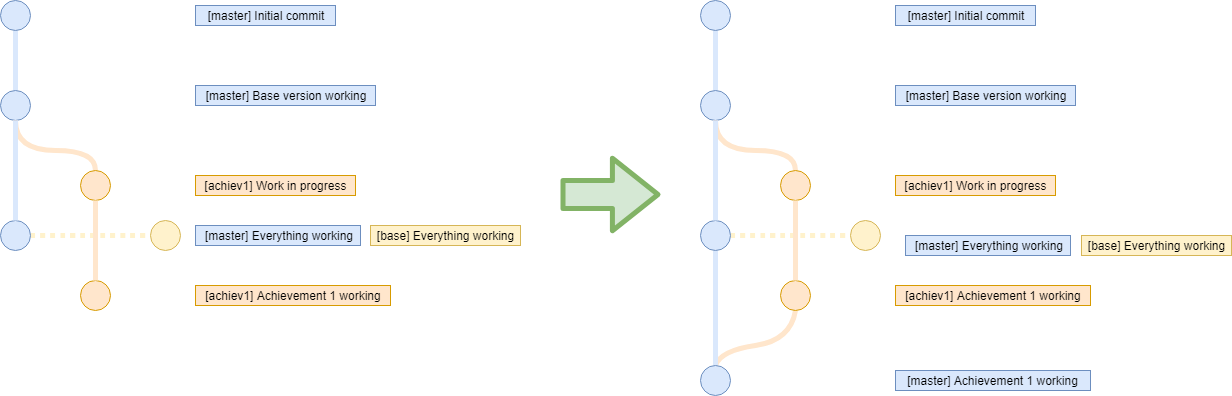
\includegraphics[scale=0.28]{branches.png}
\caption{Diagramme des branches Git, avant et après avoir passé \textbf{achiev1} sur \textbf{master}}
\label{fig:branches}
\end{figure}

% --- Améliorations possibles

\subsection{Améliorations possibles}
\label{subsct:ame_possibles}

Cependant, notre projet a beau marcher et avoir rempli les objectifs que nous nous étions fixés, différentes améliorations auraient pu être faites. Tout d'abord concernant les structures que nous avons créé. La plus flagrante serait sans doute la modélisation des singes : utiliser un tableau de singes et non pas un tableau de pointeurs de singes nous auraient permis de rendre le code plus simple et plus propre concernant le début du \textit{main} avec l'initialisation "\textit{à la va vite}".

De plus, nous aurions pu avancer un peu plus loin concernant l'avancement des achievements. Malgré le fait que nos objectifs n'étaient pas d'aller le plus loin possible mais de produire un code propre et complet, nous aurions pu faire au moins le deuxième achievement, qui à notre sens, était totalement réalisable. À noter tout de même que nos objectifs ont été atteints : nous avons bien documenté, structuré et développé notre code.

Enfin la dernière amélioration, et pas des moindres, nous pouvons améliorer notre projet en faisant en sorte d'utiliser moins de variables globales, mais plus de champs dans les structures. Certes cela rendrait les structures peut-être plus difficiles à comprendre (ou non), mais cela rendrait le code beaucoup plus clair.

% -- Compétences acquises

\subsection{Compétences acquises}
\label{subsct:competences_acquises}

Durant le développement de ce projet nous avons acquis beaucoup de compétences tant sur le plan technique que personnel. En effet nous avons appris comment gérer un projet en travaillant de manière fractionnée afin d'avoir un résultat pouvant prétendre à certaines exigences. De plus, le fait d'avoir fait un rapport et des tests complets, nous a permis de ne pas négliger l'apport que pouvait avoir une documentation remplie et structurée.

Mais nous pensons que l'apport qui a été le plus majeur a été avec l'utilisation des outils techniques. Premièrement, concernant l'utilisation de l'outil \textit{Git}. Durant nos projets à l'IUT nous avons tous deux beaucoup utilisé Git mais avec beaucoup de mauvaises manières. Nous faisions des \textit{push} avec \textit{add *}, nous ne commentions pas assez les \textit{commit} et cela se résultait par le fait que notre gestionnaire de versions était très sale. Avec ce projet, nous avons appris l'\textbf{importance} de s'organiser avec un gestionnaire de fichiers. Nous avons aussi utilisé les branches et cela de manière plus poussée qu'avant. Mais aussi comment gérer les conflits, les \textit{merge}, les problèmes de \textit{fast-forward}, etc...

De plus, l'utilisation de \textit{Emacs} et de \LaTeX nous a permis de nous familiariser avec ces outils pour le moins très puissants.

Enfin, le point technique essentiel est bien entendu, l'utilisation du langage qui nous a été bénéfique. Nous avons pu nous entraîner quant à la pratique de ce langage impératif, surtout sur l'aspect des pointeurs. Cela nous permettra certainement de mieux appréhender les langages orientés objets que nous étudierons, puisque le problème traité ici s'y serait prêté.

\end{document}
